% Deployment of the testbed on the three-node cluster used in this paper.
\documentclass[border=2pt]{standalone}
\usepackage{tikz}
\usetikzlibrary{arrows.meta,positioning,fit,calc,backgrounds}
\begin{document}
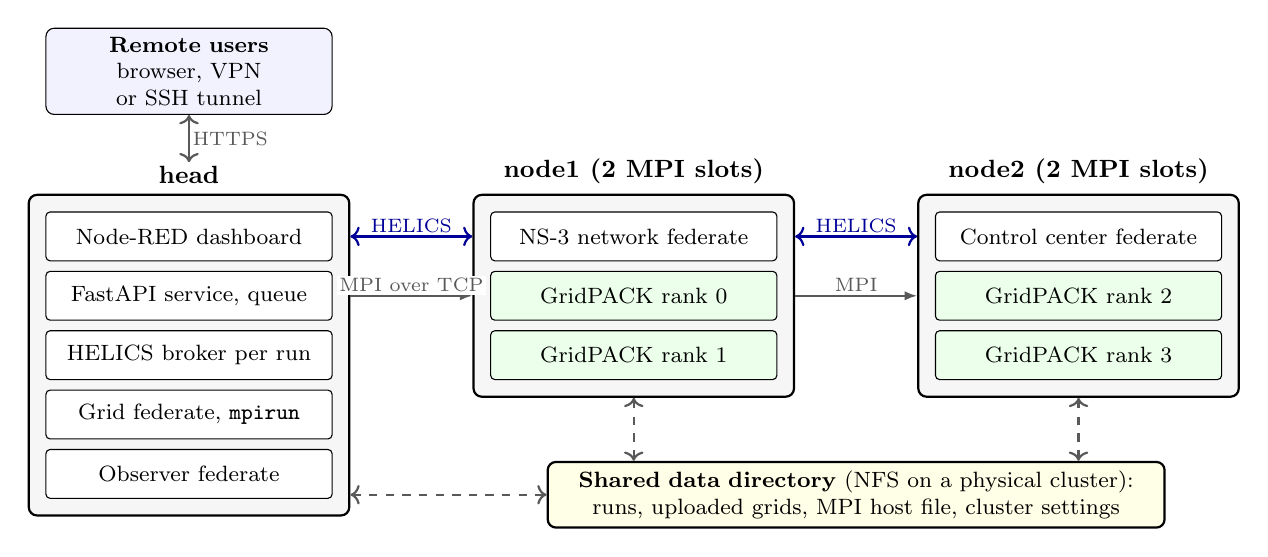
\begin{tikzpicture}[
  font=\footnotesize,
  sw/.style={draw, rounded corners=1.5pt, align=center, fill=white, text width=3.4cm, minimum height=0.62cm},
  mpi/.style={draw, rounded corners=1.5pt, align=center, fill=green!8, text width=3.4cm, minimum height=0.62cm},
  node/.style={draw, thick, rounded corners=3pt, fill=gray!7, inner sep=6pt},
  link/.style={-{Latex[length=1.6mm]}, thick, gray!70!black},
  lab/.style={font=\scriptsize, fill=white, inner sep=1pt}]
% head
\node[sw] (nr) {Node-RED dashboard};
\node[sw, below=0.12cm of nr] (api) {FastAPI service, queue};
\node[sw, below=0.12cm of api] (brk) {HELICS broker per run};
\node[sw, below=0.12cm of brk] (gf) {Grid federate, \texttt{mpirun}};
\node[sw, below=0.12cm of gf] (ob) {Observer federate};
\begin{scope}[on background layer]\node[node, fit=(nr)(api)(brk)(gf)(ob), label={[font=\small\bfseries]above:head}] (head) {};\end{scope}
% node1
\node[sw, right=2.0cm of nr] (ns) {NS-3 network federate};
\node[mpi, below=0.12cm of ns] (r0) {GridPACK rank 0};
\node[mpi, below=0.12cm of r0] (r1) {GridPACK rank 1};
\begin{scope}[on background layer]\node[node, fit=(ns)(r0)(r1), label={[font=\small\bfseries]above:node1 (2 MPI slots)}] (n1) {};\end{scope}
% node2
\node[sw, right=2.0cm of ns] (cc) {Control center federate};
\node[mpi, below=0.12cm of cc] (r2) {GridPACK rank 2};
\node[mpi, below=0.12cm of r2] (r3) {GridPACK rank 3};
\begin{scope}[on background layer]\node[node, fit=(cc)(r2)(r3), label={[font=\small\bfseries]above:node2 (2 MPI slots)}] (n2) {};\end{scope}
% shared storage
\node[draw, thick, rounded corners=3pt, fill=yellow!10, align=center, text width=7.6cm, below=0.8cm of $(n1.south)!0.5!(n2.south)$] (nfs)
  {\textbf{Shared data directory} (NFS on a physical cluster): runs, uploaded grids, MPI host file, cluster settings};
\node[draw, rounded corners=3pt, fill=blue!5, align=center, text width=3.4cm, above=1.0cm of head] (usr) {\textbf{Remote users}\\ browser, VPN or SSH tunnel};
\draw[link, <->] (usr) -- node[lab, right] {HTTPS} ([yshift=4mm]head.north);
\draw[link] (head.east |- r0) -- node[lab, above] {MPI over TCP} (n1.west |- r0);
\draw[link] (n1.east |- r2) -- node[lab, above] {MPI} (n2.west |- r2);
\draw[link, <->, blue!60!black] (head.east |- ns) -- node[lab, above] {HELICS} (n1.west |- ns);
\draw[link, <->, blue!60!black] (n1.east |- cc) -- node[lab, above] {HELICS} (n2.west |- cc);
\draw[link, <->, dashed] (head.east |- nfs.west) -- (nfs.west);
\draw[link, <->, dashed] (n1.south) -- (n1.south |- nfs.north);
\draw[link, <->, dashed] (n2.south) -- (n2.south |- nfs.north);
\end{tikzpicture}
\end{document}
